\section{Forward modelling}
\label{sec:fwd}

\subsection{Radio: from simulated maps to LoTSS}
\begin{itemize}
  \item Beam convolution, 1\,Mpc/128\,px common grid at each target's
        redshift.
  \item Noise must be beam-correlated: with white noise, real-cluster
        predictions ran to 10--27\,Gyr.
  \item Field injection into real LoTSS DR3 fields (209 downloaded, 206
        accepted at 40$'$; 202 at 80$'$) (Bruno et al.\ 2023
        precedent; Bottrell ``FullReal'' tier): real noise, sources and
        artefacts.
  \item Flux: the simulation's own predicted power, one global constant
        -- \emph{not} an observed $P_{150}$--\mfive\ anchor
        (Section~\ref{sec:flux}).
  \item Realism: image statistics vs LoTSS as separations in mock
        standard deviations (KS $p$ values inflate with sample size).

\end{itemize}
\begin{figure*}
  \centering
  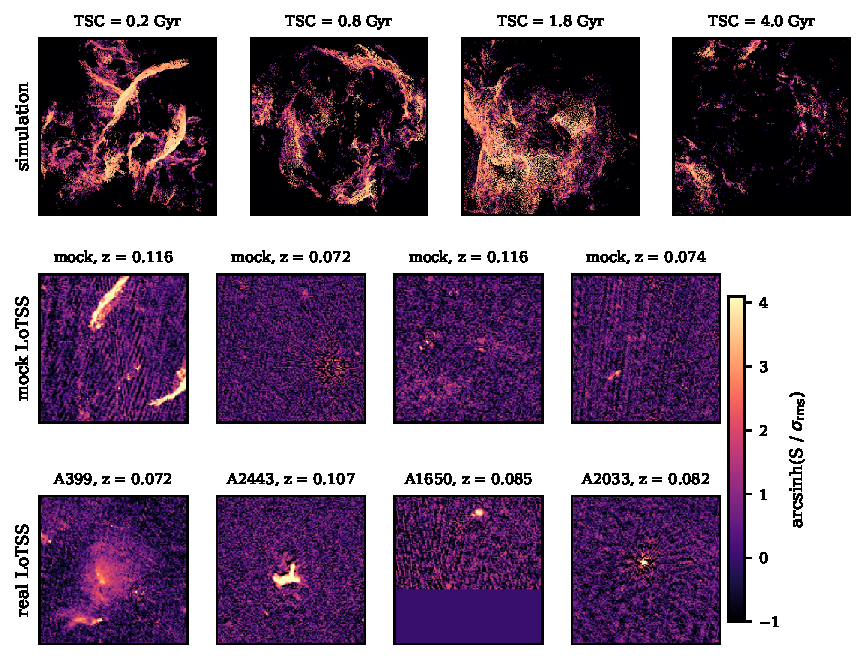
\includegraphics[width=\textwidth]{fig_radio_gallery.pdf}
  \caption{Top: simulated 144\,MHz maps (GroupPos-centred, $n_{\rm H} <
  10^{-4}$\,cm$^{-3}$ shock cells, $\pm2\,r_{500}$) for four clusters
  spanning merger time. Middle: the same clusters forward-modelled at a
  LoVoCCS redshift and injected into a real LoTSS DR3 field with the
  simulation's own flux. Bottom: real LoTSS targets on the same grid; the
  circular regions are masked compact sources.}
  \label{fig:radio_gallery}
\end{figure*}

\begin{figure*}
  \centering
  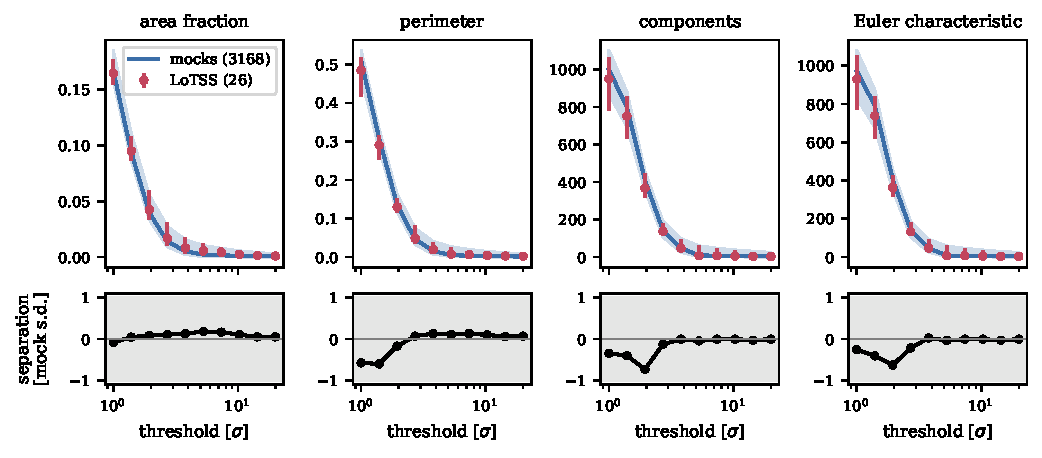
\includegraphics[width=\textwidth]{fig_radio_mf.pdf}
  \caption{Minkowski functionals of the 3168 injected mocks (band: 16--84
  per cent) against the 25 LoTSS targets (points: median and 16--84 per
  cent), at thresholds 1--20$\sigma$ of each map's noise. Bottom: the
  median offset of the real maps in units of the mock scatter. Every
  offset is at most 0.5 mock standard deviations; the largest are the
  component count and Euler characteristic at $\gtrsim$10$\sigma$, where
  compact AGN dominate.}
  \label{fig:radio_mf}
\end{figure*}

\subsection{X-ray: from 2\,Ms mocks to real Chandra depths}
\label{sec:xray}
\begin{itemize}
  \item Binomial thinning of photon counts is an exact shallower
        observation for fully exposed pixels, approximate where the mocks'
        exposure varies (chip gaps, dither edges; review F6); real archival depths (median 50\,ks all instruments,
        20\,ks ACIS-I).
  \item Sky backgrounds from soxs; particle background handled separately.
  \item Redshift placement: $1/D_L^2$ dimming, sky-area scaling of the
        background per (physically fixed) pixel, common aperture.
  \item TNG over-luminosity: mocks $\sim$3$\times$ brighter than real
        clusters (0.32 measured on Chandra; 0.28 from catalogue $L_X$);
        corrected with the catalogue value.
  \item Galactic absorption per target (small: median 2\%).
  \item Fig.~\ref{fig:lx}: the luminosity offset seen in catalogue $L_X$.
  \item Real-data processing and the particle-background normalisation
        lesson (effective-area-scaled exposure is wrong for unfocused
        background).
  \item Depth: skill saturates by $\sim$150\,ks; most real targets are
        shallower (median 31\,ks), at the steep part of the curve
        (Fig.~\ref{fig:xray_depth}).

\end{itemize}
\begin{figure}
  \centering
  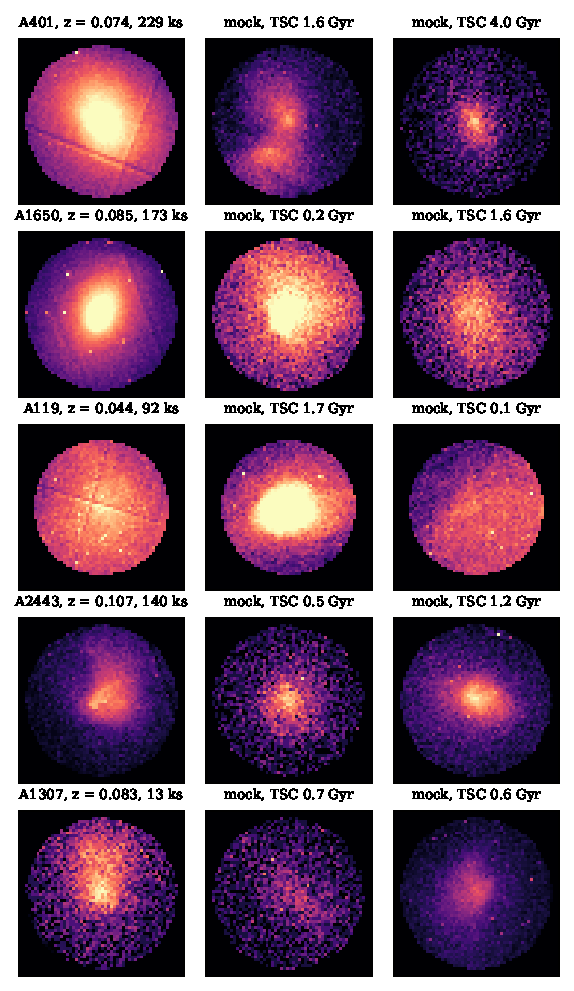
\includegraphics[width=\columnwidth]{fig_xray_gallery.pdf}
  \caption{Real Chandra ACIS-I inputs (left; particle-background
  corrected, Cycle-22-equivalent exposure) beside two mocks placed at the
  same redshift and depth, with the $L_X$ and absorption corrections.
  Pixels outside the common 8$'$ (at $z = 0.05$) aperture are zero.}
  \label{fig:xray_gallery}
\end{figure}
\begin{figure*}
  \centering
  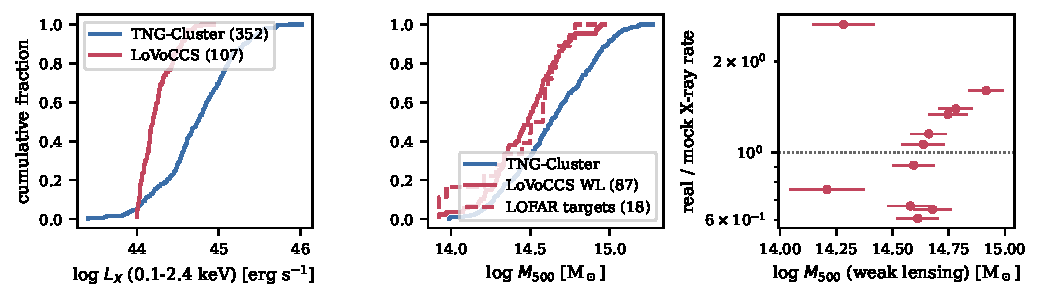
\includegraphics[width=\textwidth]{fig_lx_mass.pdf}
  \caption{Left: catalogue X-ray luminosity, TNG-Cluster against LoVoCCS
  (whose $10^{44}$\,erg\,s$^{-1}$ selection cut is visible); the medians
  differ by 0.55\,dex, a factor 3.6. Middle: $M_{500}$ of TNG-Cluster
  against LoVoCCS weak-lensing masses. Right: for the 11 Chandra targets
  with a weak-lensing mass, real X-ray count rate in the common aperture
  divided by the median of mass-matched ($\pm0.15$\,dex) mocks at the same
  redshift, after the $L_X$ correction: median 1.29, no trend with mass
  (slope $0.08 \pm 0.32$).}
  \label{fig:lx}
\end{figure*}
\begin{figure}
  \centering
  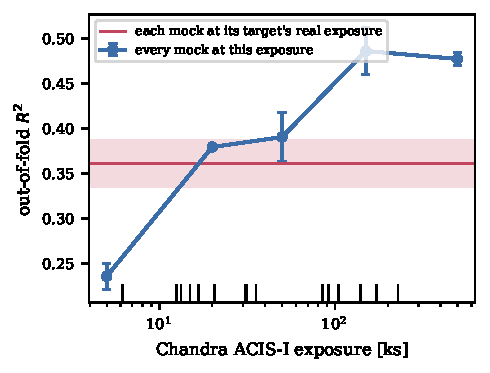
\includegraphics[width=\columnwidth]{fig_xray_depth.pdf}
  \caption{X-ray-only accuracy against exposure (mean and s.d.\ over 3
  seeds, snapshot 99): every mock placed at a target redshift with sky and
  particle backgrounds, the $L_X$ and absorption corrections, and the same
  exposure throughout. Skill rises from $R^2 = 0.24$ at 5\,ks to 0.38 at
  20\,ks and saturates near 0.48 by $\sim$150\,ks. Ticks: Cycle-22-equivalent
  exposures of the 15 real targets (median 31\,ks); the band is the model
  trained with each mock at its matching target's real exposure
  ($0.36 \pm 0.03$).}
  \label{fig:xray_depth}
\end{figure}
